\documentclass{article}
\usepackage{graphicx} % Required for inserting images
\usepackage{enumerate} %makes numbered lists
\usepackage{setspace}
\usepackage[hidelinks]{hyperref}
\usepackage{epsfig}  % for figures
\usepackage{url}  % Hyphenation of URLs.
\usepackage{lscape}  % Useful for wide tables or figures.
\usepackage[justification=raggedright]{caption}	% makes captions ragged right - thanks to Bryce Lobdell
\usepackage[labelfont=bf]{caption} % Makes the FIGURE X part of the figure caption bold
\usepackage{array} % For tables
\usepackage{multirow} %Merge multiple rows in tables
\usepackage{hhline} % for underlining table cells
\usepackage{framed} % frame around all subfigures
\usepackage{adjustbox} % custom frame around all subfigures
\usepackage{float}
\usepackage{booktabs}
\usepackage{xcolor, soul} %lets us change the text color
\usepackage{amsmath}  % for math spacing

\usepackage{enumerate}

\usepackage{geometry}
 \geometry{
 a4paper,
 total={170mm,257mm},
 left=20mm,
 top=20mm,
 }

\usepackage{hyperref}


%Commands to make the text red or blue
\newcommand{\red}[1]{\textcolor{red}{#1}}
\newcommand{\blue}[1]{\textcolor{blue}{#1}}
\newcommand{\green}[1]{\textcolor{green}{#1}}

\title{MechSE Web Reference Page - TAM 212}
\author{Melany Opolz}

\begin{document}

\maketitle
\date
\noindent Color code:
    \begin{itemize}
        \item [\textcolor{red}{\textbullet}] \red{Missing content | Reference page needs to be created}
        \item [\textcolor{blue}{\textbullet}] \blue{Specific reference page}
        \item Complete
    \end{itemize}
    
\tableofcontents

\newpage

\section{Vectors}

\subsection{Notation}

\blue{Complete reference page "vector and bases"}

\subsection{Cartesian coordinate system}
\blue{Complete in reference page "position and coordinates"}

\subsection{Polar coordinate system}
\blue{Complete in reference page "position and coordinates"}

\subsection{Units}
\blue{Complete in reference page "position and coordinates"}

\subsection{Unit vectors}
\blue{Complete in reference page "vector and bases"}

\subsection{Vectors bases}
\blue{Complete in reference page "vector and bases"}

\subsection{Changing bases}
\blue{Complete in reference page "vector and bases"}

\subsection{Projection and complementary projection}
\blue{Complete in reference page "vector and bases"}

\subsection{Change in length and direction}
\blue{Complete in reference page "Vector calculus"}

\subsection{Spherical Coordinates}
\blue{Complete in reference page "Spherical coordinates"}

\subsection{\red{Applications}}
    \subsubsection{\red{Spin lunch}}
    \red{This was mentioned in lecture but no actual example was given. It would be a good idea to include it.} Application for "Polar coordinates".

    \subsubsection{\red{Haystack antenna}}
    \red{This is mentioned in L09-Notes, slide 2. This topic needs to be formally expanded. Refer to Fig \ref{fig:AppAnetnna} }. Application for "Change of basis".
    \begin{figure}[h!]
        \centering
        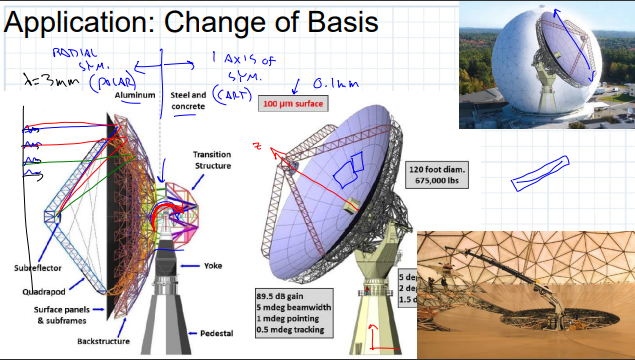
\includegraphics{VectorsFigs/AppAntenna.png}
        \caption{From L09-Notes, slide 2}
        \label{fig:AppAnetnna}
    \end{figure}
    
    \subsubsection{Shortest flight paths}
    \blue{Complete in reference page "Shortest flight paths"}. Application for Spherical coordinates.




\newpage
\section{Vector Calculus}

\subsection{Dot product}
\red{*This topic appears in 2 reference pages*} \\
\blue{Complete in reference page "vector and bases"} \\
\blue{Explained in reference page "vector identities"}

\subsection{Cross product}
\red{*This topic appears in 2 reference pages*} \\
\blue{Complete in reference page "vector and bases"} \\
\blue{Explained in reference page "vector identities"}

\subsection{Derivatives}
    \subsubsection{Cartesian}
    \blue{Complete in reference page "vector calculus"} \\
    \red{The example in Fig\ref{Fig:CartesianDerivatives} could be added:}
\begin{figure*}[!h]
\centering
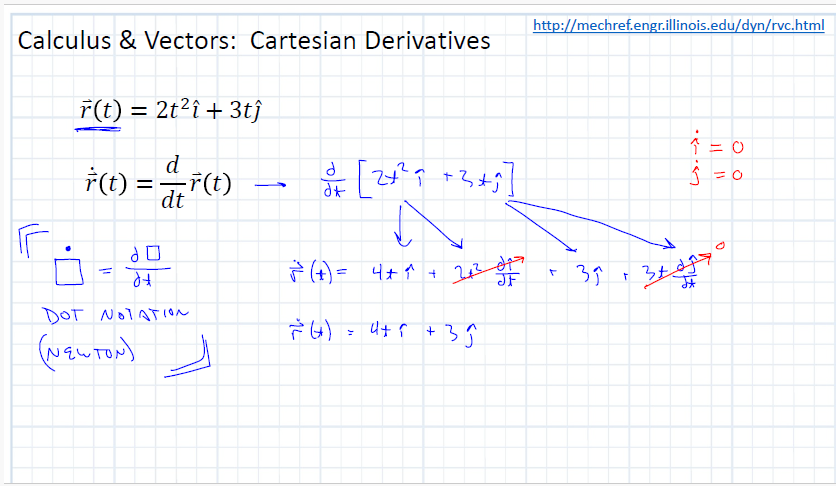
\includegraphics[width=0.9\textwidth]{VectorCalculusFigures/Cartesian Derivatives.png}
\vspace{-2mm}
\caption{\small Taken from L03-Notes, slide 6.}
\vspace{-3mm}
\label{Fig:CartesianDerivatives}
\end{figure*}
    
    \subsubsection{\red{Non-Cartesian: Polar basis}}
    \red{An example like in Fig\ref{Fig:Non-CartesianPolarBasis} could be added in "vector and bases"} 
\begin{figure*}[h!]
\centering
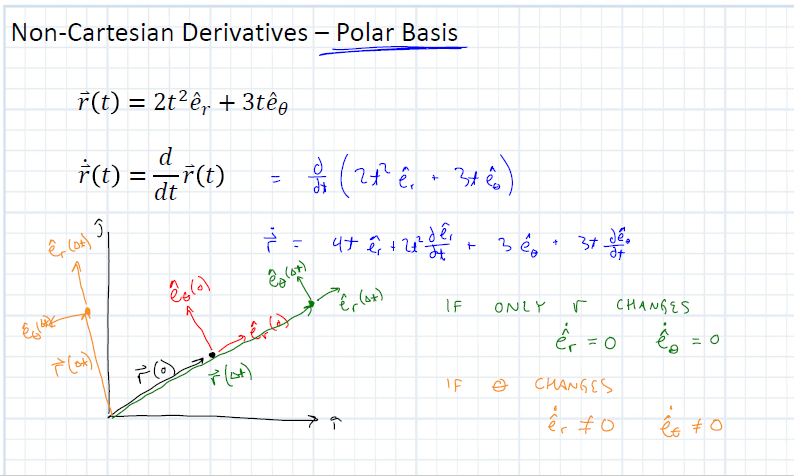
\includegraphics[width=0.9\textwidth]{VectorCalculusFigures/Non-Cartesian Polar Basis.png}
\vspace{-2mm}
\caption{\small Taken from L03-Notes, slide 7.}
\vspace{-3mm}
\label{Fig:Non-CartesianPolarBasis}
\end{figure*}
    
    \subsubsection{\red{Graphical estimation}}
        \red{The information in Fig \ref{Fig:GraphicalEstimation} could be included as a new section in "vector and bases"} 
\begin{figure*}[h!]
\centering
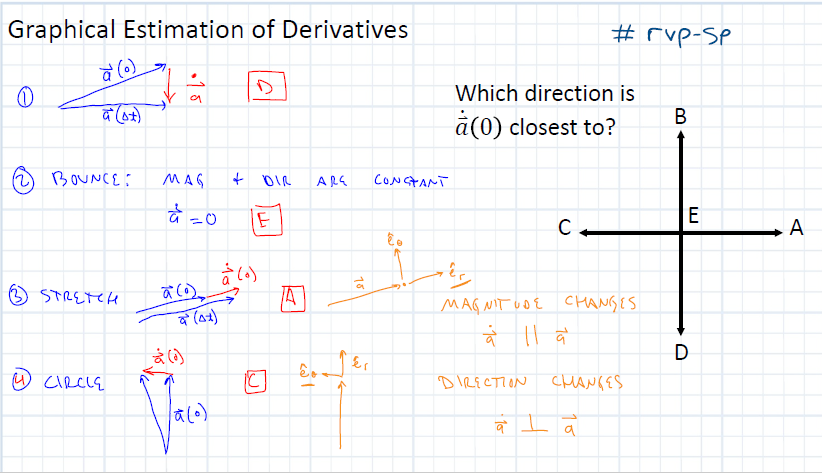
\includegraphics[width=0.9\textwidth]{VectorCalculusFigures/Graphical Estimation of Derivatives.png}
\vspace{-2mm}
\caption{\small Taken from L03-Notes, slide 8.}
\vspace{-3mm}
\label{Fig:GraphicalEstimation}
\end{figure*}

\subsection{Chain rule}
    \subsubsection{Scalars}
    \blue{Complete in "Vector Calculus"}
    \subsubsection{Second derivative}
    \blue{Complete in "vector Calculus"}
    
\subsection{\red{Integration}}
\red{Include summary of both Polar and Cartesian integration as in Fig \ref{fig:SummaryVecInt}}
\begin{figure}[h!]
    \centering 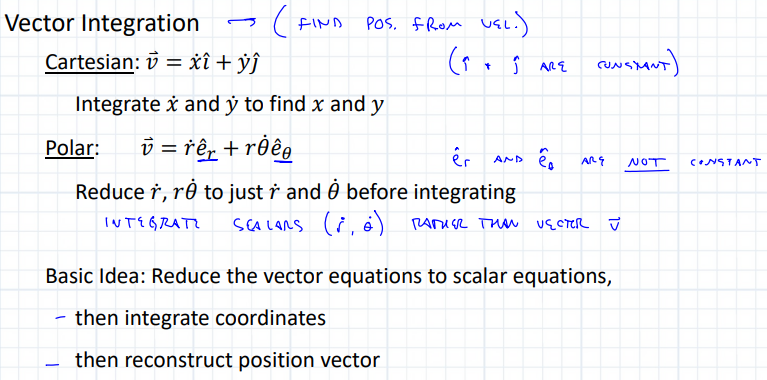
\includegraphics[width=0.8\textwidth]{VectorCalculusFigures/SummaryVectorIntegration.png}
    \caption{From L08-Notes, slide 6}
    \label{fig:SummaryVecInt}
\end{figure}
    \subsubsection{Cartesian basis}
    \blue{Complete in "Vector calculus"}
    \subsubsection{\red{Polar basis}}
    \red{Add the information in Fig \ref{fig:PolarIntegration}}
    
    \begin{figure}[h!]
        \centering 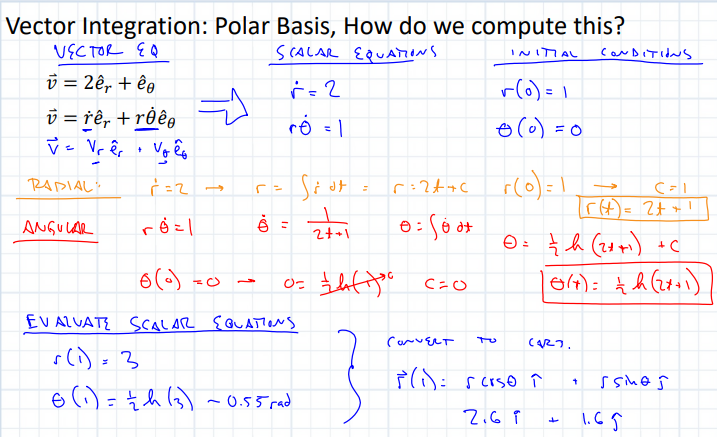
\includegraphics[width=0.8\textwidth]{VectorCalculusFigures/PolarIntegration.png}
        \caption{From L08-Notes, slide 5} \label{fig:PolarIntegration}
    \end{figure}

\subsection{\red{Solving equations}}
\red{Include step by step on how to solve vector equations as shown in Fig \ref{fig:SolvingEqnsSteps}}

\begin{figure}[h!]
    \centering 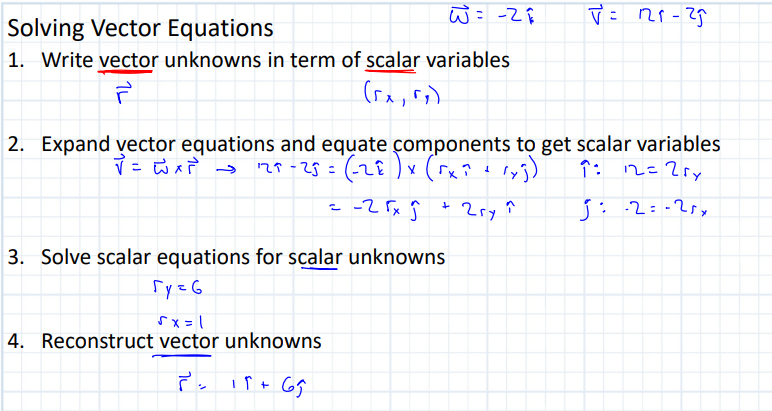
\includegraphics[width=0.8\textwidth]{VectorCalculusFigures/SolvingEqnsSteps.png}
    \caption{From L09-Notes, slide 10}
    \label{fig:SolvingEqnsSteps}
\end{figure}


Include examples as shown in Figs \ref{fig:SolvingEqns}, \ref{fig:SolvingEqns2} 

\begin{figure}[h!]
    \centering 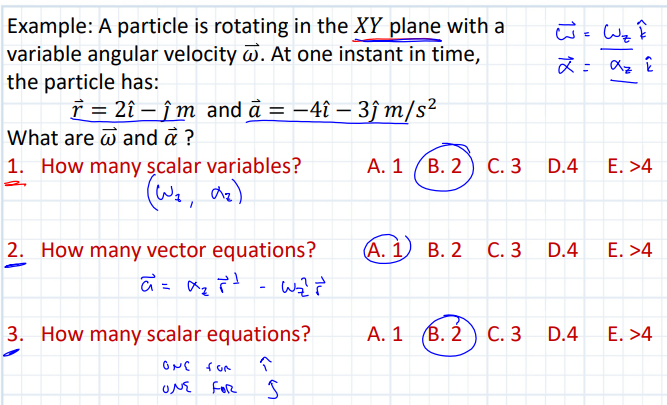
\includegraphics[width=0.8\textwidth]{VectorCalculusFigures/SolvingEqns.png}
    \caption{From L09-Notes, slide 9}
    \label{fig:SolvingEqns}
\end{figure}

\begin{figure}
    \centering 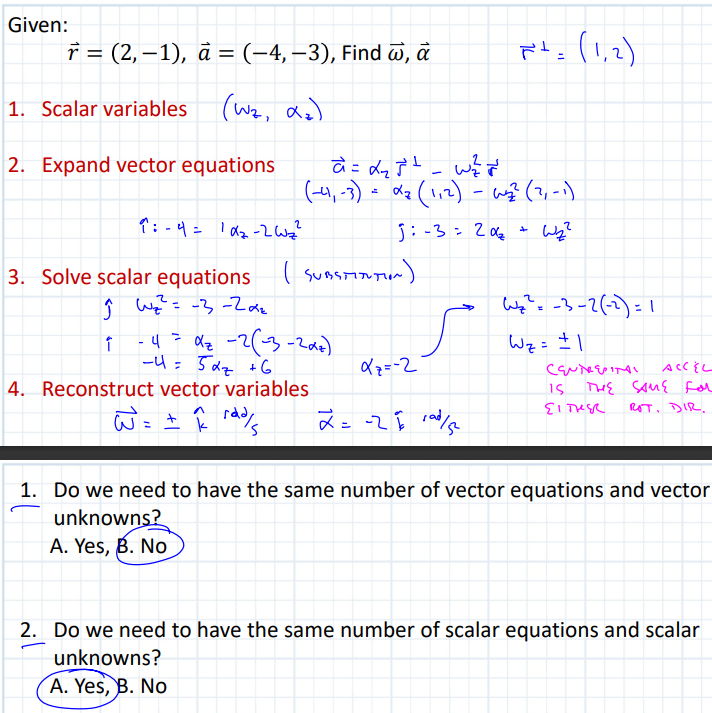
\includegraphics[width=0.8\textwidth]{VectorCalculusFigures/SolvingEqns2.png}
    \caption{From L10-Notes, slides 5-6}
    \label{fig:SolvingEqns2}
\end{figure}
\section{Particle Kinematics}

\subsection{Position, velocity, acceleration}
\blue{Complete in  "Position, velocity, and acceleration"}\\
\red{Add the table summary shown in Fig \ref{fig:PosVelAcce}}

\begin{figure}[h!]
    \centering
    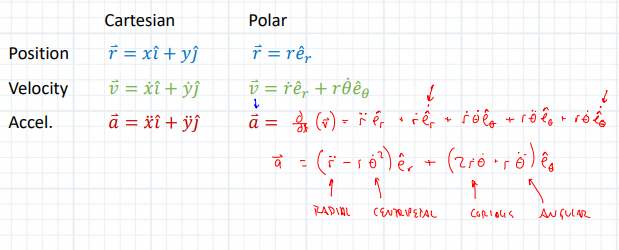
\includegraphics[width=0.9\textwidth]{ParticleKinematicsFigs/PosVelAcce.png}
    \caption{From L07-Notes, slide 2}
    \label{fig:PosVelAcce}
\end{figure}

    \subsubsection{Graphical understanding}
    \blue{Complete in reference page "Position, velocity, and acceleration"} \\

\subsection{Rotating frames}
    \subsubsection{Angular velocity}
    \blue{Complete in reference page "Rotations and angular velocity"} \\
    \subsubsection{Angular acceleration}
        \blue{Complete in reference page "Position, velocity, and acceleration"} \\
        \red{This equation is displayed under the title "Velocity and acceleration in polar basis". Add the description of each term as shown in Fig \ref{fig:AngularAccelerationEq}}
    \begin{figure}[h!]
        \centering   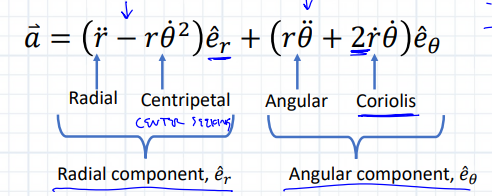
\includegraphics[width=0.6\textwidth]{ParticleKinematicsFigs/AngularAcceleration.png}
        \caption{From L08-Notes, Slide 2}
        \label{fig:AngularAccelerationEq}
    \end{figure}
    
\subsection{Tangential}
    \subsubsection{Normal basis}
    \blue{Complete in reference page "Tangential/normal basis"} \\
    \subsubsection{Normal and Tangential acceleration}
        \blue{Complete in reference page "Tangential/normal basis"} \\
    \subsubsection{Curvature}
        \blue{Complete in reference page "Tangential/normal basis"} \\

\subsection{\red{System comparison: Cartesian/Polar/Tangent-Normal}}
\red{Add summary table as in Fig \ref{fig:SystemsComparison}}

\begin{figure} [h!]
    \centering
    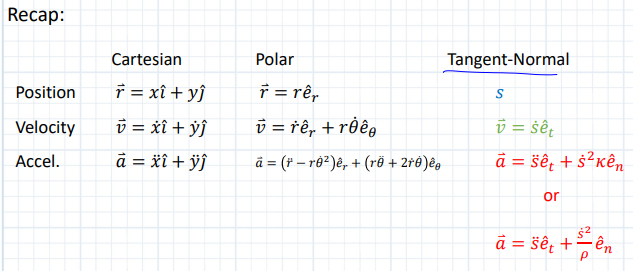
\includegraphics[width=0.9\textwidth]{ParticleKinematicsFigs/SystemsComparison.png}
    \caption{From L12-Notes, slide 3}
    \label{fig:SystemsComparison}
\end{figure}

\subsection{\red{Applications}}
    \subsubsection{\red{Train wheels}}
    \red{This was mentioned in lecture but it was not expanded. It would be a great idea to include a picture or example.} Refers to "angular velocity".
    
    \subsubsection{\red{Variable inertia flywheel}}
    \red{This is mentioned in L07-Notes, Slide 6. This paper is cited \url{https://doi.org/10.1016/j.egyr.2020.01.001}. This picture is included \ref{fig:AppFlywheel}.} Refers to "Angular accelerations".
    \begin{figure}[h!]
        \centering
        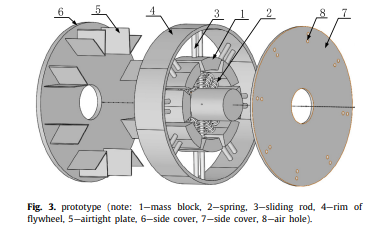
\includegraphics{ParticleKinematicsFigs/AppFlywheel.png}
        \caption{From L07-Notes, slide 6.}
        \label{fig:AppFlywheel}
    \end{figure}
    
    \subsubsection{Celestial velocities}
    \blue{Complete in "Celestial Velocities".} Refers to "angular velocity" and "angular acceleration".
    
    \subsubsection{Track transition curves}
    \blue{Complete in "Track transition curves".} Refers to "position, velocity, and acceleration" and "Tangential".

    \subsubsection{\red{Roller coaster}}
    \red{This topic needs to be created, it was mentioned in lecture with no information or figure}
\section{Particle Kinetics}

\subsection{Classical mechanics}
\blue{Complete in "Kinetics of point masses"}
    \subsubsection{Method of assumed forces and method of assumed motion}
    \blue{Complete in "Kinetics of point masses"}
    \subsubsection{Solution steps}
    \blue{Complete in "Kinetics of point masses"}
    \blue{More information about Free body diagrams included in "Free boy diagrams"}

\subsection{\red{Numerical integration}}

\red{Add information shown in Fig \ref{fig:NumericalIntegration}}

\begin{figure}[h!]
    \centering 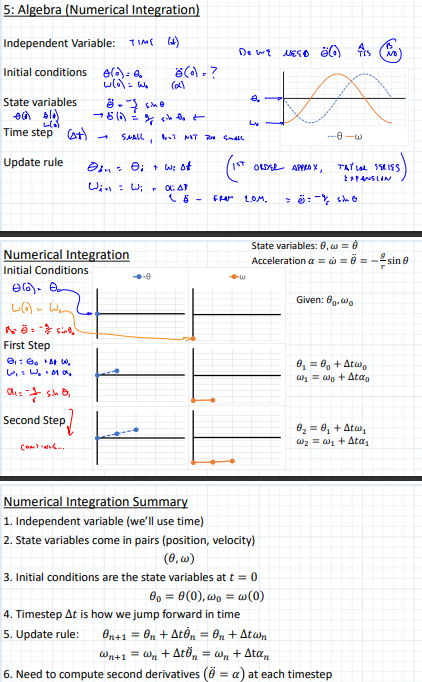
\includegraphics{ParticleKinetics/NumericalIntegration.png}
    \caption{From L14-Notes, slides 7-9}
    \label{fig:NumericalIntegration}
\end{figure}

\subsection{\red{Applications}}
    \subsubsection{\red{Kiiking}}
    \red{This topic is in L13-Notes, slides 9-10. Include information in Fig \ref{} and this YouTube link \url{https://www.youtube.com/shorts/qvW0sz4kBLQ}}. Application for "Particle kinetics".

    \begin{figure}[h!]
        \centering
        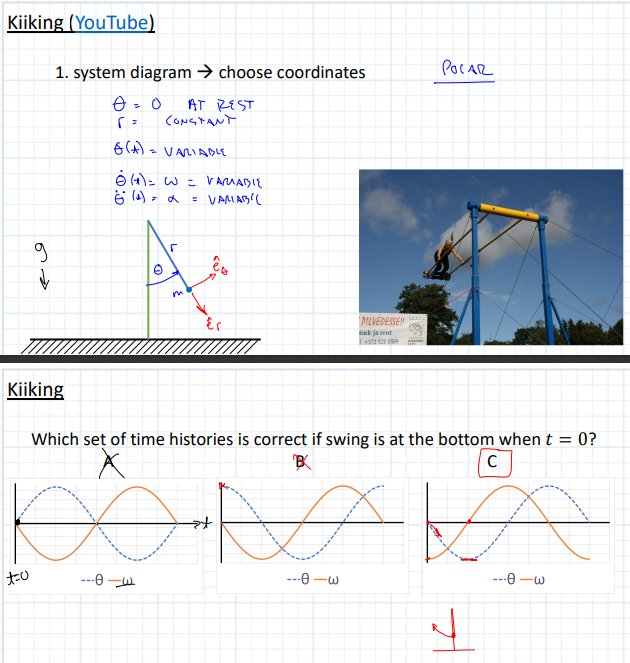
\includegraphics{ParticleKinetics/AppKiiking.png}
        \caption{From L13-Notes, slides 9-10.}
        \label{fig:AppKiiking}
    \end{figure}

    \subsubsection{Accelerating and braking}
    \label{sub:PartKin_acce}
    \blue{Complete in "Accelerating and braking". Just the introduction and the information under "Point mass model".} 

    \subsubsection{Banked turns}
    \label{sub:PartKin_turns}
    \blue{Complete in "Banked turns". Just the introduction and the information under "Track geometry" and "Point mass model".} 

    \subsubsection{Projectiles with air resistance}
    \blue{Complete in "Projectiles with air resistance".} 
\section{Rigid Body Kinematics}

\subsection{Rigid bodies}
\blue{Complete in "Rigid bodies"}

\subsection{Rotating rigid bodies}
\blue{Complete in "Rigid bodies"}

\subsection{Rigid body velocity}
\blue{Complete in "Rigid bodies"}

\subsection{Constrained motion}
\blue{Complete in "Constraints and constrained motions"}

\subsection{Rigid body acceleration}
\blue{Complete in "Rigid bodies"}

\subsection{\red{Gears}}
\red{Include the information in Fig \ref{fig:GearsRecap}  as a broad introduction to the topic}

\begin{figure}[h!]
    \centering
    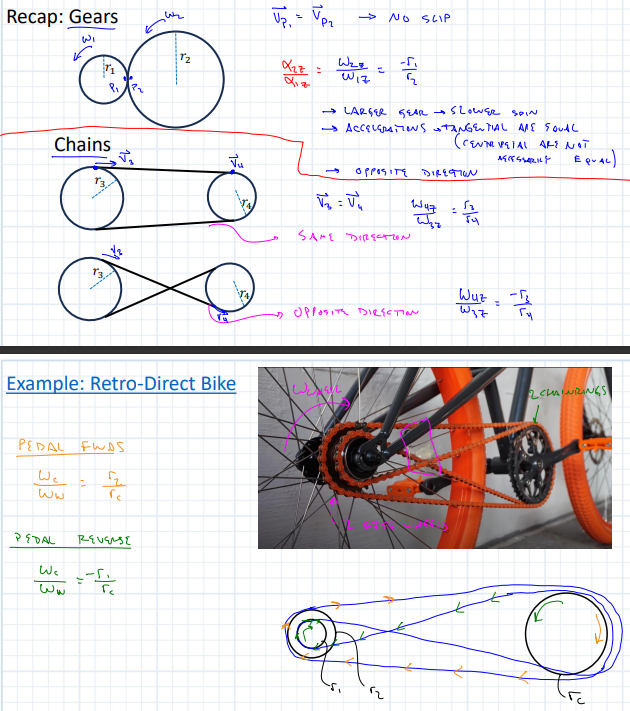
\includegraphics{RigidBodyKinematics/GearsRecap.png}
    \caption{From L21-Notes, slide 2}
    \label{fig:GearsRecap}
\end{figure}

    \subsubsection{\red{Standard sign convention}}
    \red{Add information shown in Fig \ref{fig:gears}}
    \begin{figure}[h!]
        \centering
        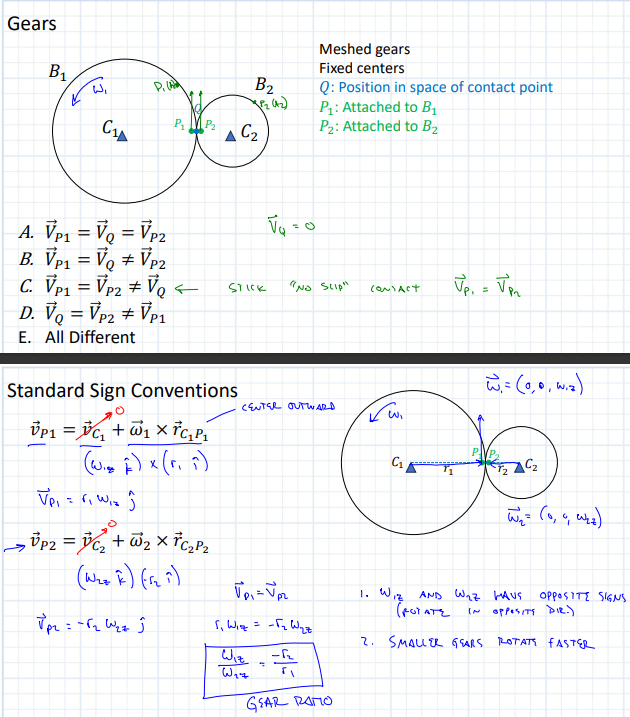
\includegraphics{RigidBodyKinematics/Gears.png}
        \caption{From L20-Notes, slides 4-5}
        \label{fig:gears}
    \end{figure}

\noindent \red{Include animation of examples as the ones in Fig \ref{fig:GearsExamples}}

    \begin{figure}[h!]
         \centering  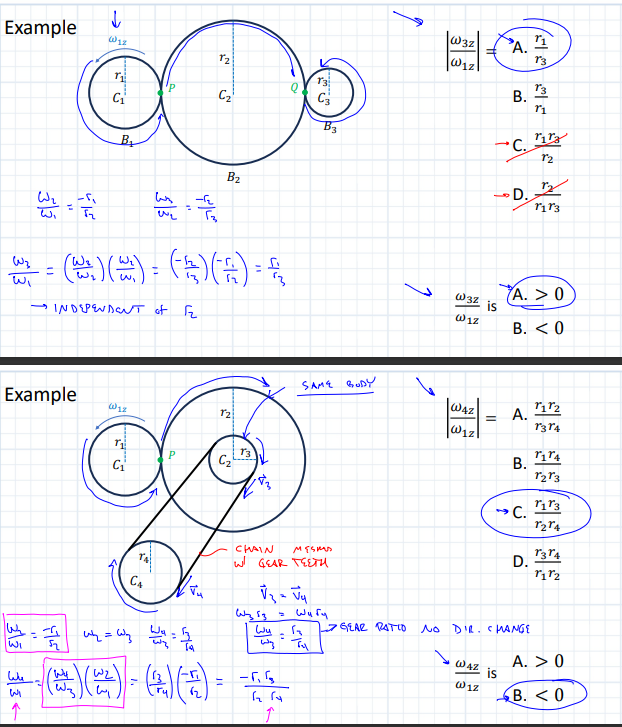
\includegraphics{RigidBodyKinematics/GearsExamples.png}    
         \caption{From L20-Notes, slides 7-8}
         \label{fig:GearsExamples}
    \end{figure}

    \subsubsection{\red{Accelerations in contact (no slip)}}
    \red{Add the information included in Fig \ref{fig:GearsAcceleration}}

    \begin{figure}[h!]
        \centering 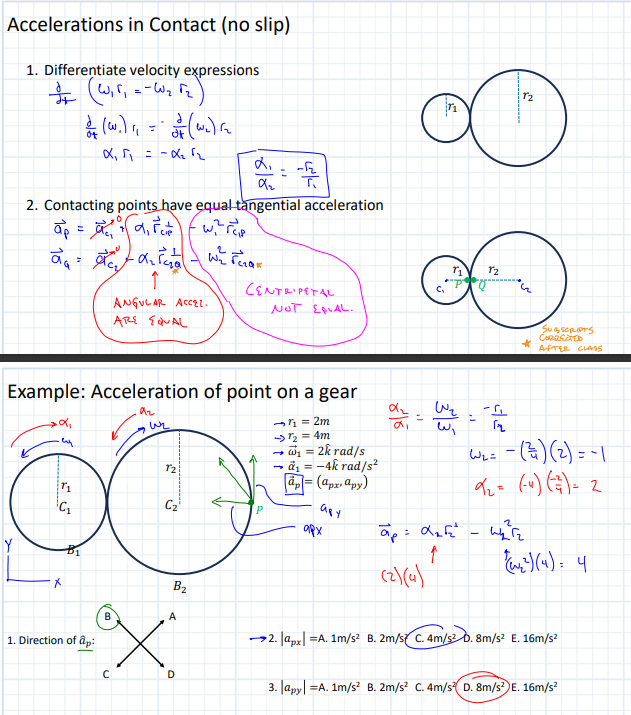
\includegraphics{RigidBodyKinematics/GearsAcceContact.png}
        \caption{From L20-Notes, slides 9-10}
        \label{fig:GearsAcceleration}
    \end{figure}
    
\subsection{\red{Applications}}
    \subsubsection{\red{Train passenger comfort}}
    \red{This topics need to be clearly organized and expanded. Refer to Fig \ref{fig:AppTrainPassenger}}. Application for "Rigid body acceleration".

    \begin{figure}[h!]
        \centering
        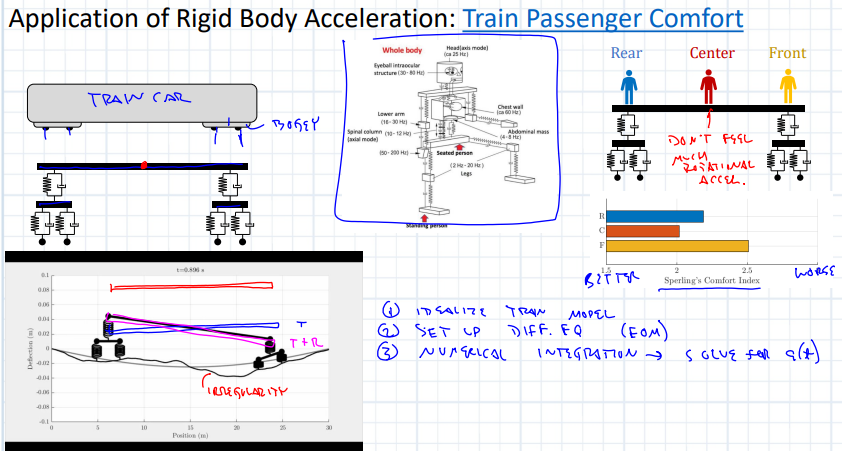
\includegraphics{RigidBodyKinematics/AppTrainPassenger.png}
        \caption{From L19-Notes, slide 2.}
        \label{fig:AppTrainPassenger}
    \end{figure}

    \subsubsection{Steering geometry}
    \blue{Complete in "Steering geometry".} This refers to "Rigid Bodies".

    \subsubsection{Knee Joint}
    \blue{Complete in "Four-Bar Linkages" under the subtitle "Example: Knee joint (constrained motion)".} This refers to "Constrained motion".

    \subsubsection{Suspensions with Watt's linkage}
    \blue{Complete in "Four-Bar Linkages" under the subtitle "Example: Suspensions with Watt's linkage (constrained motion)".} This refers to "Constrained motion".

    \subsubsection{\red{Aerobie Orbiter}}
    \red{This topic was mentioned in lecture but it was not expanded.} Application for "Rigid body rotation".


\section{Rigid Body Kinetics}

\subsection{\red{Center of mass (COM)}}
\blue{Complete in "Center of mass"} 

\noindent \red{Add to this section the information shown in Fig \ref{fig:COM}}

\begin{figure}[h!]
    \centering 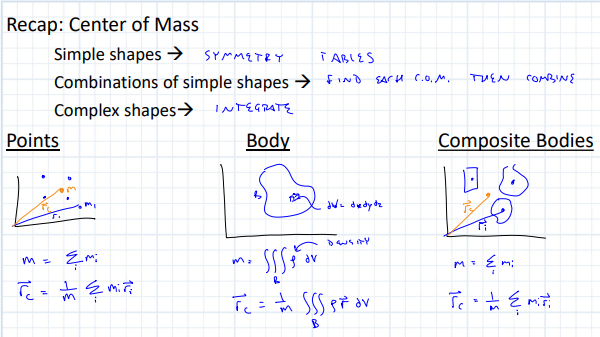
\includegraphics{RigidBodyKineticsFigs/CenterofMass.png}
    \caption{From L12-Notes, slide 2}
    \label{fig:COM}
\end{figure}

\subsection{Mass moment of inertia}
\blue{Complete in "Moments of Inertia"} 

\subsubsection{Parallel axis theorem}
\blue{Complete in "Moments of Inertia"} 
 
\subsubsection{Additive theorem}
\blue{Complete in "Moments of Inertia"} 

\subsection{\red{Instantaneous centers}}
\red{Add this information:}
\begin{itemize}
    \item \red{For a rigid body moving in 2D (rotating and possibly translating)}
    \item \red{Instantaneous Center “M” is the point on or off the rigid body that has zero
velocity at that instant (i.e. no translation at this point)}
    \item \red{Point that the body rotates about (at that instant in time)}

\end{itemize}

\red{Add some examples as shown in Figs \ref{fig:ICexamples1}, \ref{fig:ICexamples2}}

\begin{figure}[h!]
    \centering 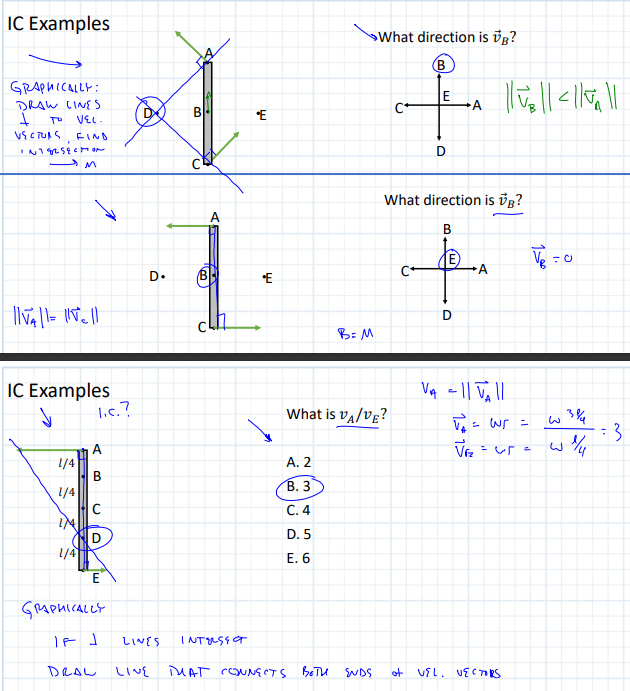
\includegraphics{RigidBodyKineticsFigs/ICexamples1.png}
    \caption{From L25-Notes, slides 5-6}
    \label{fig:ICexamples1}
\end{figure}

\begin{figure}[h!]
    \centering 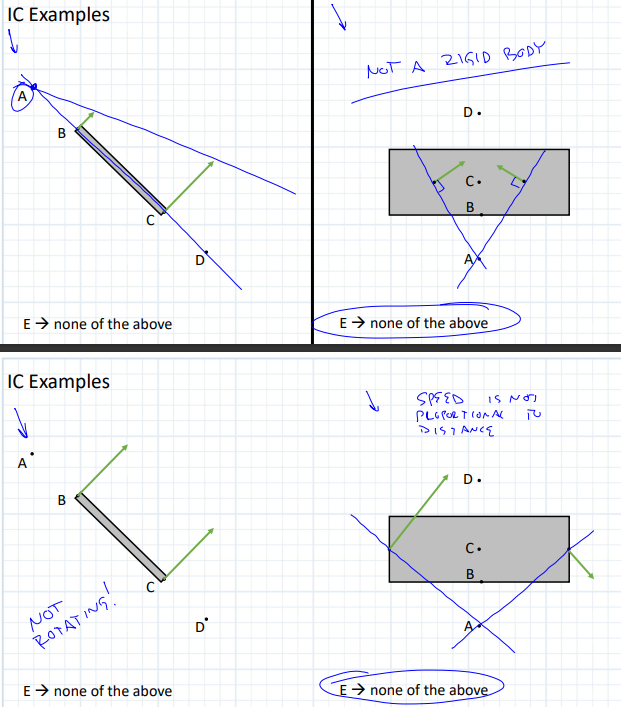
\includegraphics{RigidBodyKineticsFigs/ICexamples2.png}
    \caption{From L25-Notes, slides 8-9}
    \label{fig:ICexamples2}
\end{figure}

\red{Add: Graphical rules for finding (M) (Instantaneous Center) as shown in Fig\ref{fig:ICgraphRules}}

\begin{figure}[h!]
    \centering 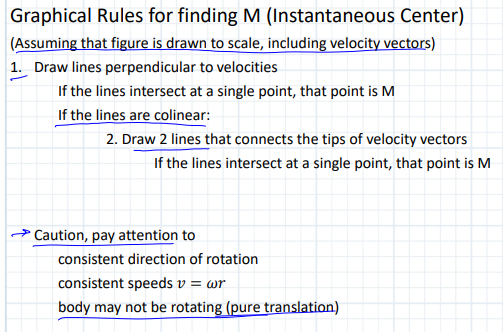
\includegraphics{RigidBodyKineticsFigs/ICgraphicalRules.png}
    \caption{From L25-Notes, slide 10}
    \label{fig:ICgraphRules}
\end{figure}

\subsection{\red{Applications}}
    \subsubsection{\red{Cargo Ships}}
    \red{This topic is in L22-Notes, slides 3-4, refer to Fig \ref{fig:AppCargoShip}}. Application for "Center of mass".

    \begin{figure}[h!]
        \centering
        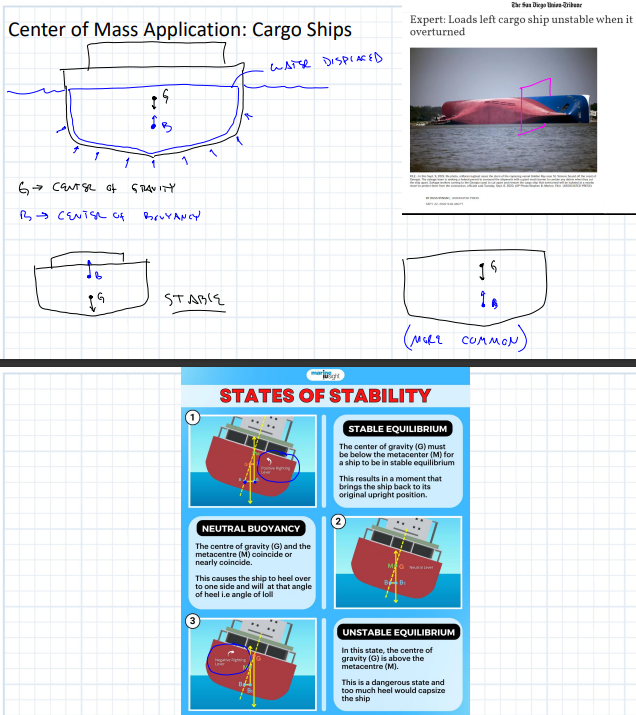
\includegraphics{RigidBodyKineticsFigs/AppCargoShip.png}
        \caption{From L22-Notes, slides 3-4.}
        \label{fig:AppCargoShip}
    \end{figure}

    \subsubsection{Tuned Mass Damper}
    \red{This topic is in L24-Notes, slide 9, include the information in Fig \ref{fig:AppCargoShip}, and this link to a YouTube video \url{https://www.youtube.com/watch?v=GzMuF-LMGaM} }. Application for "Rigid body kinetics".

    \begin{figure}[h!]
        \centering
        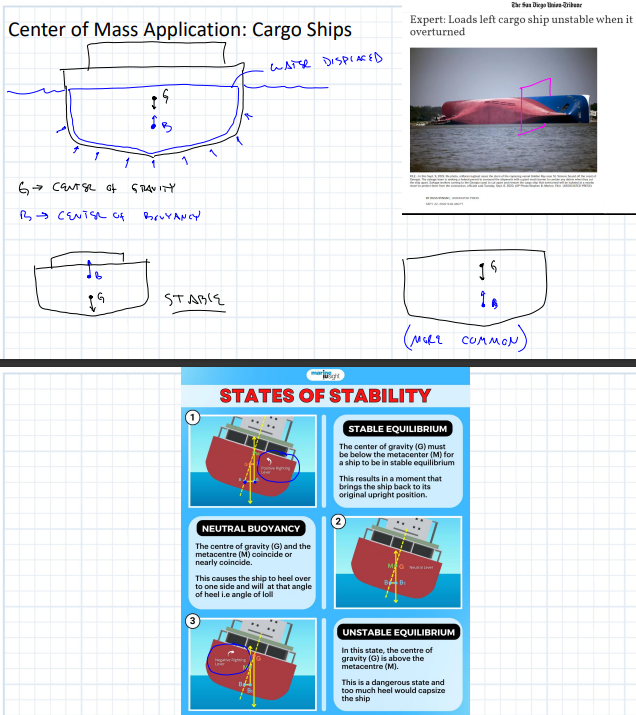
\includegraphics{RigidBodyKineticsFigs/AppCargoShip.png}
        \caption{From L24-Notes, slide 9.}
        \label{fig:AppCargoShip}
    \end{figure}

    \subsubsection{Accelerating and braking}
    \blue{Complete in "Accelerating and braking". Include all the information starting at "2D rigid body model".} Refer back to  \ref{sub:PartKin_acce}

    \subsubsection{Banked turns}
    \blue{Complete in "Banked turns". Include all the information starting at "2D rigid body model".} Refer back to  \ref{sub:PartKin_turns}
\section{Contact and Rolling}

\subsection{Rigid bodies in contact}
\blue{Complete in "Rolling motion"}

\subsection{Rolling motion}
\blue{Complete in "Rolling motion"}

\subsection{Rolling on curved surfaces}
\blue{Complete in "Rolling motion"}

\subsection{\red{Applications}}
    \subsubsection{\red{Bearings}}
    \red{This topic is in L27, slides 13-14, include information in Fig \ref{fig:AppBearings}. Pictures are from this book \url{https://i-share-uiu.primo.exlibrisgroup.com/permalink/01CARLI_UIU/gpjosq/alma99955068260305899}}. Application for "Rolling on curved surfaces".

    \begin{figure}[h!]
        \centering
        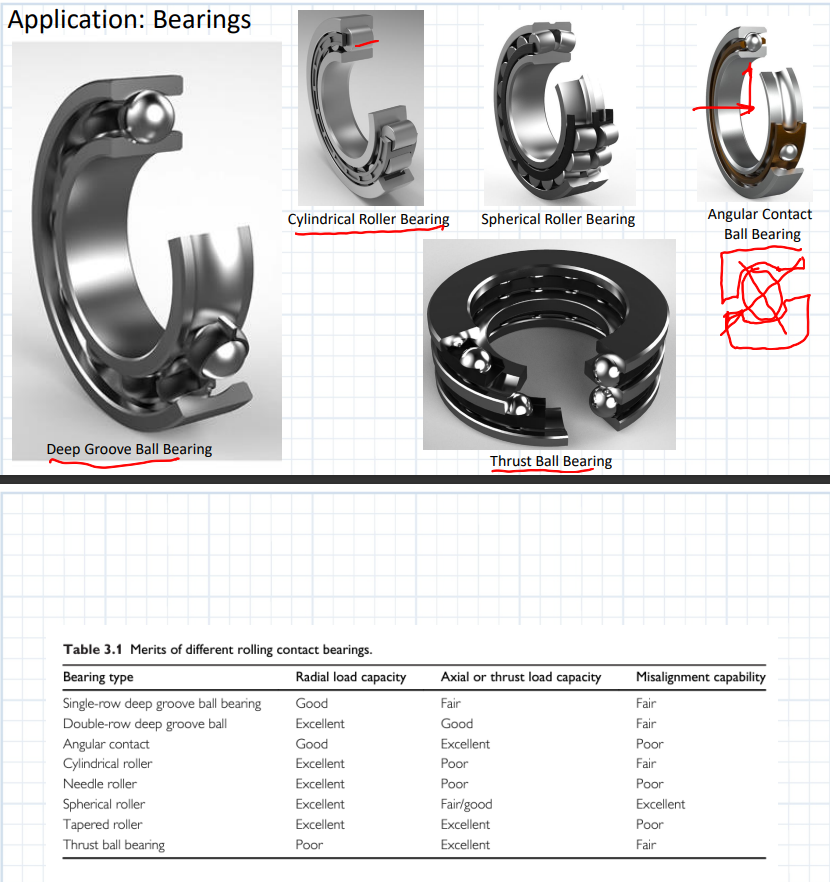
\includegraphics{ContactRollingFigs/AppBearings.png}
        \caption{From L27, slides 13-14}
        \label{fig:AppBearings}
    \end{figure}


\section{Work and Energy}

\subsection{\red{Energy}}
\blue{Mostly complete in "Energy and work".}

\noindent \red{Add information as shown in Fig \ref{fig:Energy}. Equations of potential gravitational and elastic are already included in reference page}

\begin{figure}[h!]
    \centering 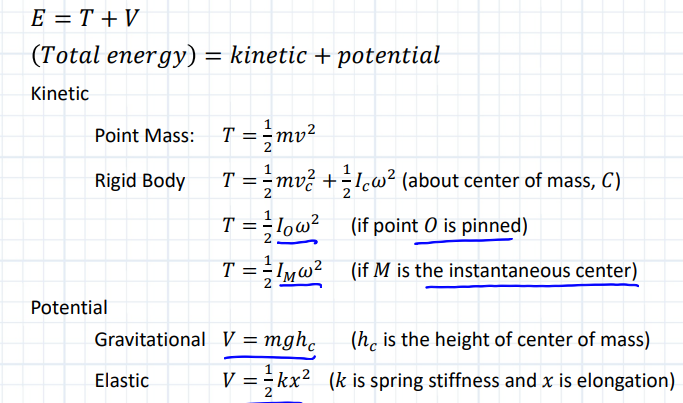
\includegraphics[width=0.8\textwidth]{WorkEnergyFigs/Energy.png}
    \caption{From L29-Notes, Slide 8}
    \label{fig:Energy}
\end{figure}

\subsection{Work}
    \subsubsection{\red{Work-Energy}}
    \red{Include equation and description shown in Fig \ref{fig:WorkEnergy}}
    \begin{figure}[h!]
    \centering 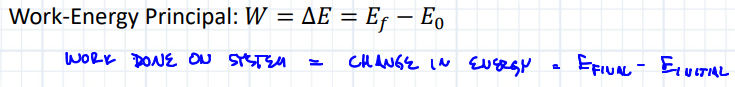
\includegraphics[width=0.8\textwidth]{WorkEnergyFigs/WorkEnergy.png}
    \caption{From L29-Notes, Slide 9}
    \label{fig:WorkEnergy}
\end{figure}

    \subsubsection{\red{Work done by a Force}}
    \blue{Complete in "Energy and work"}

    \noindent \red{Include example shown in Fig \ref{fig:WorkExample}}
    \begin{figure}[h!]
    \centering 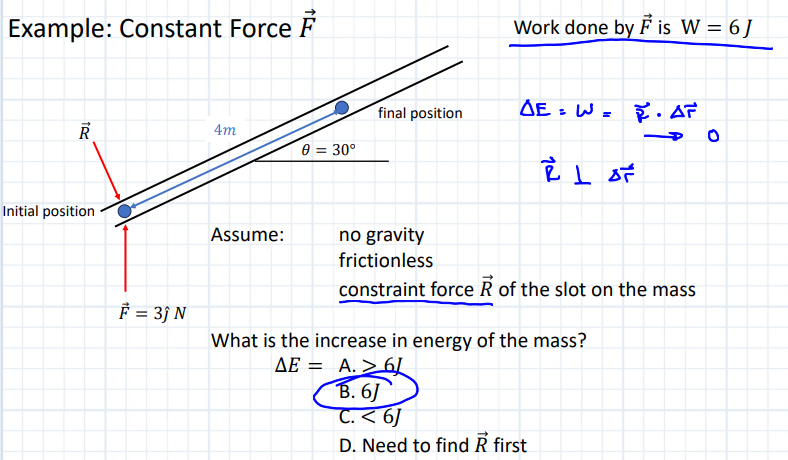
\includegraphics[width=0.85\textwidth]{WorkEnergyFigs/WorkExample.png}
    \caption{From L30-Notes, slide 6}
    \label{fig:WorkExample}
\end{figure}

    \subsubsection{Conservative vs Non-conservative forces}
    \blue{Complete in "Energy and work"}

    \subsubsection{\red{Work done by Friction}}
    \red{Add information and example shown in Fig \ref{fig:WorkFriction}}
    \begin{figure}[h!]
    \centering 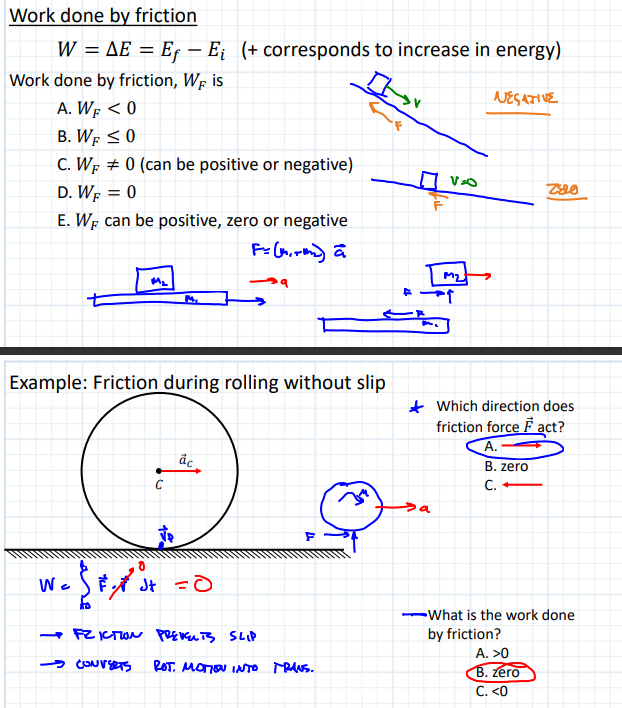
\includegraphics[width=0.85\textwidth]{WorkEnergyFigs/WorkFriction.png}
    \caption{From L30-Notes, slides 11-12}
    \label{fig:WorkFriction}
    \end{figure}
    
    \subsubsection{\red{Work done by a Moment}}
    \red{Add information and example shown in Fig \ref{fig:WorkMoment}}
    
    \begin{figure}[h!]
    \centering 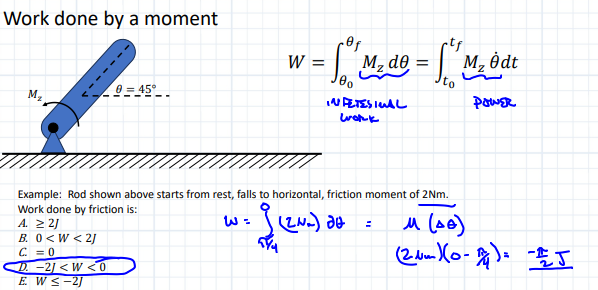
\includegraphics[width=0.85\textwidth]{WorkEnergyFigs/WorkMoment.png}
    \caption{From L30-Notes, slide 13}
    \label{fig:WorkMoment}
    \end{figure}
    
\subsection{Friction}
    \subsubsection{Stick, Transition, Slip}
    \red{Add information shown in Fig \ref{fig:Friction}}
    
    \begin{figure}[h!]
    \centering 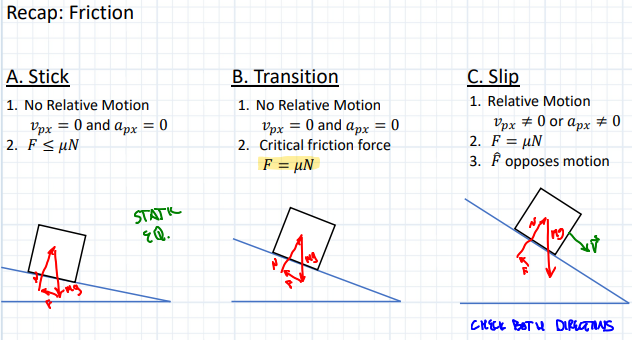
\includegraphics[width=0.85\textwidth]{WorkEnergyFigs/Friction.png}
    \caption{From L33-Notes, slide 2}
    \label{fig:Friction}
    \end{figure}
    
    \subsubsection{Solution procedure}
    \red{Add information shown in Fig \ref{fig:FrictionSolutionProcedure}}
    
    \begin{figure}[h!]
    \centering 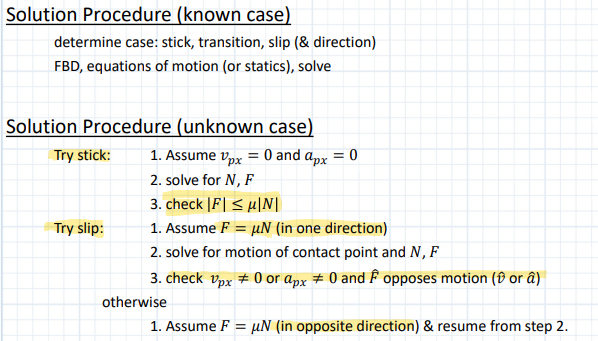
\includegraphics[width=0.85\textwidth]{WorkEnergyFigs/FrictionSolutionProcedure.png}
    \caption{From L30-Notes, slide 13}
    \label{fig:FrictionSolutionProcedure}
    \end{figure}

\subsection{\red{Momentum}}
\red{Add short summary like in Fig \ref{fig:Momentum} at the end of the section}
    \begin{figure}[h!]
    \centering 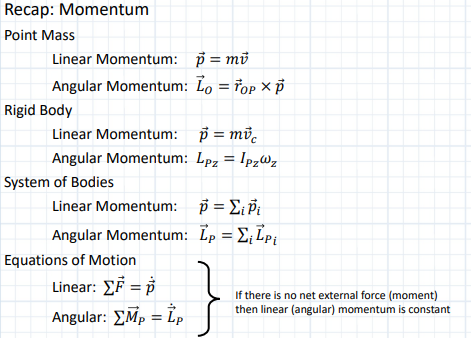
\includegraphics[width=0.85\textwidth]{WorkEnergyFigs/Momentum.png}
    \caption{From L31-Notes, slide 11}
    \label{fig:Momentum}
    \end{figure}
    
    \subsubsection{of a point mass}
    \blue{Complete in "Momentum, impulse and collisions"}
    
    \subsubsection{of a rigid body}
    \blue{Complete in "Momentum, impulse and collisions"}
    
    \subsubsection{of a system of rigid bodies}
    \blue{Complete in "Momentum, impulse and collisions"}

\subsection{Impulse}
\blue{Complete in "Momentum, impulse and collisions"}

\subsection{\red{Applications}}
    \subsubsection{\red{Wind Turbine}}
    \red{This is included in L29-Notes, slides 11-12. Include the information in Fig \ref{fig:AppWindTurbine}.} Application for "Energy".
    
    \begin{figure}[h!]
    \centering 
    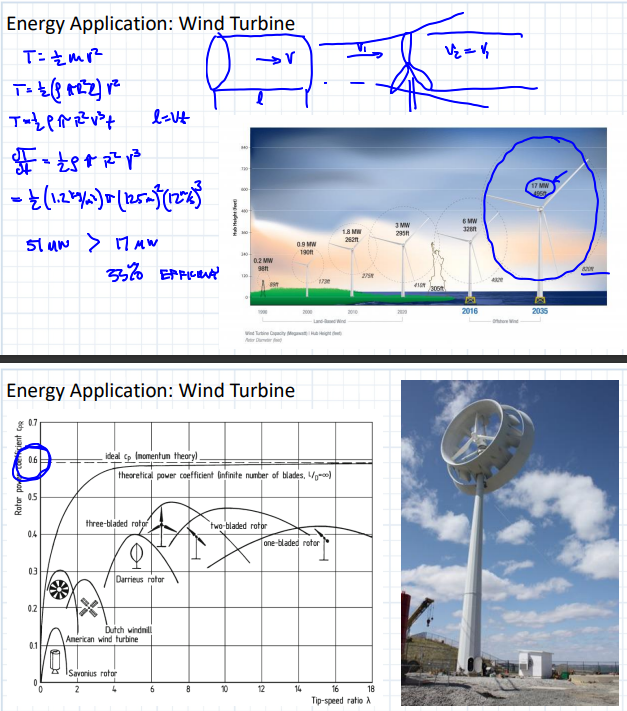
\includegraphics{WorkEnergyFigs/AppWindTurbine.png}
    \caption{From L29-Notes, slides 11-12}
    \label{fig:AppWindTurbine}
    \end{figure}
    
    
    \subsubsection{\red{Race Cars}}
    \red{This is included in L33-Notes, slides 11-12. Include the information in Fig \ref{fig:AppRaceCars}.} Application for "Friction".
    
    \begin{figure}[h!]
    \centering 
    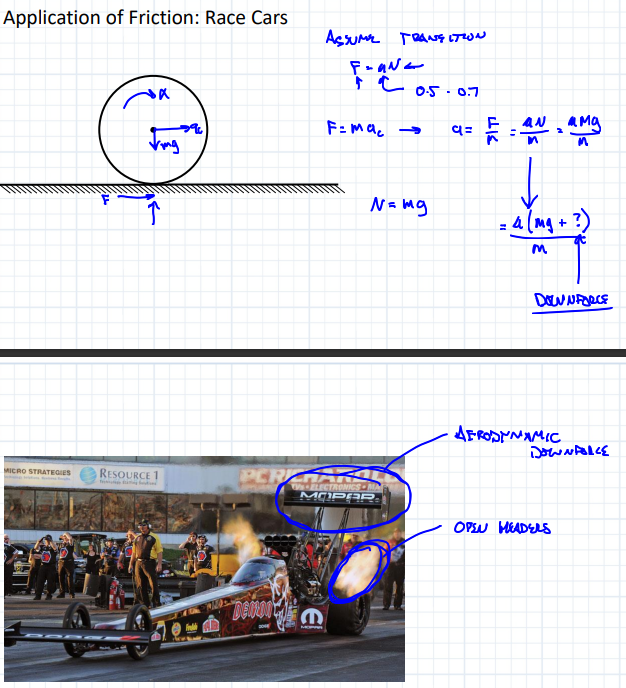
\includegraphics{WorkEnergyFigs/AppRaceCars.png}
    \caption{From L33-Notes, slides 11-12}
    \label{fig:AppRaceCars}
    \end{figure}
\section{Questions to ask Instructor}

\begin{itemize}
    \item Overall organization in categories and order of topic appearance. I followed lecture notes, which differed a little bit from current reference pages.
    \item Application sections. The ones in red need include the overall idea but I need an instructor to make the decision on what information, pictures, equations should be included in the reference page. Also:

        \begin{enumerate}
        \item In the reference page, under Application, there is a full reference page named "Four-Bar Linkages". I am not sure to which topic each subtitle should be linked. I only referenced "Example: Knee joint (constrained motion)", "Example: Suspensions with Watt's linkage (constrained motion)" to "rigid body kinematics - Constrained motion".
        \item In the reference page, under Application, there is a full reference page named "Projectiles with air resistance". I am not sure to which topic each subtitle should be linked. As for now, they are under "Applications" of "Particle Kinetics" as "Projectiles with air resistance".
\end{enumerate}
    
\end{itemize}




\end{document}
